%%%%%%%%%%%%%%%%%%%%%%%%%%%%%%%%%%%%%%%%%%%%%%%%%%%%%%%%%%%%%%%%%%%%%%%%
% RevTeX 4.1 LaTeX
% Kevin C. Young
% Scalable & Secure Systems Research (08961)
% Thu Mar  5 15:29:19 PST 2015
%%%%%%%%%%%%%%%%%%%%%%%%%%%%%%%%%%%%%%%%%%%%%%%%%%%%%%%%%%%%%%%%%%%%%%%%

\documentclass[aps,nofootinbib,pra,notitlepage,twocolumn]{revtex4-1}

\usepackage{amsfonts,amsmath,amssymb,amsthm}
\usepackage{array,bm,color}
\usepackage{epsfig,graphicx,nomencl,revsymb4-1,upgreek,url}
\usepackage{hyperref}
\usepackage{algorithm}
\usepackage{algpseudocode}
\hypersetup{colorlinks=true, pdfauthor=Kevin C. Young, pdftitle=}
%\hypersetup{citecolor={blue}, colorlinks={true}, filecolor={blue},
%   linkcolor={blue}, pdfauthor=, pdfkeywords= pdfsubject=, pdftitle=,
%   urlcolor{blue}}



\newcommand{\tr}{{\rm Tr\thinspace}}
\newcommand{\bra}[1]{\ensuremath{\left\langle{#1}\right\vert}}
\newcommand{\ket}[1]{\ensuremath{\left\vert{#1}\right\rangle}}
\newcommand{\braket}[2]{\left\langle #1 | #2 \right\rangle}
\newcommand{\ketbra}[2]{\left| #1 \right\rangle\!\!\!\,\left\langle #2 \right|}
\newcommand{\abs}[1]{\left\vert #1 \right\vert}
\newcommand{\expect}[1]{\ensuremath{\left\langle{#1}\right\rangle}}
\newcommand{\timeorder}{\ensuremath{\underset{\leftarrow}{\mathcal{T}}}}
\newcommand{\ident}{{\mathbb1}}
\newcommand{\order}[1]{\mathcal{O}\left( #1 \right)}
\newcommand{\diag}[1]{\mathrm{diag}\{#1\}}
\newcommand{\trans}[1]{#1^\mathsf{T}}
\newcommand{\T}{\mathsf{T}}

\newcommand{\erf}[1]{Eq.~(\ref{#1})}
\newcommand{\needcite}{{\color{blue}\textsuperscript{[citation needed]}}}
\newcommand{\note}[1]{{\color{red}[#1]}}
\newcommand{\kcy}[1]{{\color{red}[#1]_{\rm{KCY}}}}

%-------------Header begins here----------------------------------------
\begin{document}
\title{Decorrelating Errors in Quantum Gates by Random Gate Synthesis}

\author{Anthony Polloreno}
% \email[Email: ]{apolloreno}
\affiliation{Rigetti Computing, Berkeley, CA}

\author{Kevin C. Young}
\email[Corresponding author: ]{kyoung@sandia.gov}
\affiliation{Sandia National Laboratories, Livermore, CA}

\date{\today}

\begin{abstract}
Thresholds for fault-tolerant quantum computation are often calculated assuming a noise model in which errors are uncorrelated. While convenient for simulation, these error models are often unphysical. Recent work by Preskill and others has shown that arbitrarily long computations may be performed even in the presence of spatial correlation, provided the correlation is sufficiently weak and decays sufficiently quickly with distance, but at the cost of a significantly lower threshold. The success of algebraic decorrelation methods, such as dynamical decoupling, demonstrate that quantum control techniques are capable of reducing temporal noise correlations. We propose to introduce similar methods to effect the spatial decorrelation of errors in quantum circuits, thereby increasing the threshold for fault-tolerant computation in such systems.
\end{abstract}

\pacs{}

\maketitle

\section{Introduction}

%Thresholds for fault-tolerant quantum computation are often calculated assuming a noise model in which errors are uncorrelated. While convenient for simulation, these error models are often unphysical.  Recent work by Preskill and others has shown that the arbitrarily long computations may be performed even in the presence of spatial correlation, provided the correlation is sufficiently weak and decays sufficiently quickly with distance, but at the cost of a significantly lower threshold. The success of algebraic decorrelation methods, such as dynamical decoupling, demonstrate that quantum control techniques are capable of reducing temporal noise correlations. We propose to introduce similar methods to effect the spatial decorrelation of errors in quantum circuits, thereby increasing the threshold for fault-tolerant computation in such systems.  

Steady progress has been made in the theory of quantum error correction, proving higher thresholds for increasingly general models of noise \cite{Aharonov2006}. These results show that quantum computation is feasible, however recent NISQ \cite{Preskill2018} devices have noise that is not only often above thresholds, but that also violates assumptions made by the models used in proofs.

As an example, many models assume that errors are local, however systems can have spatially correlated error on more than two qubits that arise from multi-qubit terms in the Hamiltonian, such as:
\begin{equation}\label{eq:0}
  H(t) = \sum_{n}\sum_{i}\sum_{j=x,y,z} a^{\textbf{i}}_{\textbf{j}}(t)(\sigma_{j_1}^{i_1}\otimes\sigma_{j_2}^{i_2}\otimes ... \otimes \sigma_{j_n}^{i_n})
\end{equation}
where $a^{\textbf{i}}_{\textbf{j}}$ is a stochastic process. In a standard nearest-neighbors topology, like those found in super-conducting qubit architectures, these terms might arise from an effective model where high-frequency degrees of freedom are intergrated out to yield high-weight operators. These noise channels are one way in which the assumptions used in proofs of thresholds may be violated.

Another assumption that is instrumental in proving many threshold theorems is Markovianity \cite{Kitaev1997}. There are many ways in which devices can behave in non-Markovian ways, and NISQ devices have already been shown to be subject to drift in controls, \cite{Kelly2018} and in general non-Markovian noise \cite{BlumeKohout2017}. Other authors have tried to address these problems \cite{Wallman2016, Campbell2017, Heim2016} by using circuit composition to try to remove correlated noise. [WHY IS WHAT WE'RE DOING BETTER?]

To remedy these problems, we take a different approach and propose to inject additional decorrelating randomness into the system through the use of \emph{balanced control solutions} (BCSs). BCSs are families of control solutions that all approximate the same target gate, but with balanced errors for any given instance of the noise Hamiltonian. That is, for a target gate, $U_T$, we seek a family of control solutions, $c_i(t)$, each implementing an approximation $U_i$ to the target gate, such that the family of unitary approximations is \emph{balanced}. A balanced family is one which satisfies, for some small $\alpha$,
\begin{equation}\label{eq:1}
  \frac{1}{N}\sum_{i=1}^N \omega_i U_i \rho U_i^\dagger = DPN[\alpha]\left(U_T \rho U_T^\dagger \right)
\end{equation}

Where $DPN[\alpha](\rho)$ is a \textit{generalized} depolarizing noise channel with strength $\alpha$. (For the rest of this paper, we will refer to them just as depolarizing channels.) Such a channel is defined as:
\begin{equation}\label{eq:2}
  DPN[\alpha](\rho) \rightarrow (1-\alpha)\rho + \alpha\sum p_i \sigma_i\rho\sigma_i
\end{equation}
with $p_i$ summing to one. This means that on average, the unitary approximations implement the target unitary followed by a small depolarizing channel. The task of constructing the BCSs will fall to optimal control.

This techique can be used to turn coherent error into incoherent error and correlated error into uncorrelated error. The former gives the benefit that the error incurred from incoherent errors compound linearly, while coherent errors compound quadratically. The latter gives the benefit of reducing non-Markovian effects. This is a particularly useful property of BCSs, as diagnosing non-Markovianity in a gateset is challenging, but essential to perform reliable quantum computation. Many routines exist that can assess the quality of a gateset, however in the presence of non-Markovianity most of them become unreliable.

For example, randomized benchmarking and tomography will report incorrect answers without any syndrome, [CITATION NEEDED], and gateset tomography will report that the gateset failed to be Markovian, but will fail to diagnose in what way it was non-Markovian. Because BCSs change the error to a depolorizing channel, the correlations in the noise can be massively reduced, and the process can be made much closer to Markovian, at no real cost to the fidelity of the implemented gate.

\section{GRAPE}\label{GRAPE}
Generating BCSs can be done in a variety of ways, using any quantum optimal control technique \cite{Caneva2011, Machnes2018} to find a family of controls. For simplicity in this paper we use the GRAPE algorithm to generate candidate pulseshapes to approximate the target gate. First described in \cite{Khaneja2005}, the GRAPE (GRadient Ascent Pulse Engineering) algorithm is a technique for finding piecewise constant control sequences that approximate a desired unitary, $U_T$. Defining our uncontrolled Hamiltonian as $H_0$, our control Hamiltonians as $H_{i\neq 0}$, and our \textit{control matrix} $u_{ij}$ as containing control amplitude associated with the $i^{th}$ time step and the $j^{th}$ hamiltonian, we can write our approximate unitary at any timestep as
\begin{equation}\label{eq:3}
  U_i = \exp\{-i\Delta t(H_0 + \sum_{j=1}^{n}u_{ij}H_{ij}\}
\end{equation}
Then, to measure the simularity of our approxiate unitary $U_n$, and our target unitary $U_T$, we can define a cost function $J(U) = Tr\{U_T^{\dagger}U_n\}$.

To optimize this cost function we can perform the following standard update loop for some threshold value $\varepsilon > 0$ and step size $\delta > 0$:
\begin{algorithm}[H]
\floatname{algorithm}
  \caption{\textsc{\textbf{Gradient Ascent}}}
  \begin{algorithmic}
    \While{$J(U_n) < (1-\varepsilon$)}
    \State $u_{ij} \rightarrow u_{ij} + \delta\frac{\partial J(U)}{\partial u_{ij}}$
    \For{$1 \leq i \leq n$}
    \State $U_i \rightarrow \exp\{-i\Delta t(H_0 + \sum_{i=0}^{n}u_{ij}H_i)\}$
    \EndFor
    \State $U \rightarrow \prod_1^nU_i$
    \EndWhile 
  \end{algorithmic}
\end{algorithm}

In general these gradients can be computed by propagating partial derivatives of the cost function with respect to control parameters through each timestep of the  via the chain rule. However, in \cite{Khaneja2005} Khaneja et al. derive a simple update formula that is correct to first order. In particular one can show that:
\begin{align}
\frac{\partial J(U)}{\partial u_{ij}} = -2Re\{\braket{{U_{j+1}^{\dagger}...U_N^{\dagger} U_T}}{i\Delta tH_jU_j...U_1}\\
\braket{U_j...U_1}{U_{j+1}^{\dagger}...U_N^{\dagger} U_T}\} +  \mathcal{O}(\Delta t^2)
\end{align}

In this paper we have modified the update step to use instead use approximately the following gradient:
\begin{align}\label{quadrature}
\int p(\vec{\delta})\frac{\partial J(U(\vec{\delta}))}{\partial u_{ij}} d\vec{\delta}
\end{align}
with $p(\vec{\delta})$ Gaussian distributed. This technique has been used in previous works such as \cite{Goerz2014} to ensure that the optimal control results are robust over a wide range of errors, and we approximate this integral approximately in this paper by using Gaussian quadrature. Doing this ensures that the family of controls produced by our routine perform moderately well over a range of stochastic errors.

\section{Optimal Control Problem}\label{ocp}
\subsection{Random Gate Synthesis}
To explore the utility of BCSs, we consider the following Hamiltonian:
\begin{equation}\label{eq:2}
  H(t) = H_0 + \sum_{i=1}^n (c_i(t) + \delta_i(t))H_i
\end{equation}
for control Hamiltonians $H_i$, free evolution Hamiltonian $H_0$ and time-varying random variables $\delta_i$. Such a model might describe a superconducting qubit quantum processor where control amplitudes for the RF pulses vary over time. Correlations between different $\delta_i$ might arise if two of the controls have the same noise source. Examples of shared noise sources include $X$ and $Y$ gates in superconducting qubit architectures might use the same AWG and pulse envelope, and diurnal temperature drift of control electronics.
\subsection{Channel Approximation}
After using GRAPE or another optimal control routine to synthesize a collection of controls, we must find the weights $w_i$ such that the collection of controls form a BCS as described in (\ref{eq:1}). To do this, for each control $U_i$ we find the unitary error channel $\mathcal{E}_i$ such that $\mathcal{E}_iU_i=U_T$, where $U_T$ is the target gate. If we consider the Pauli-Liouville representation of this error channel, the diagonal terms are the \textit{stochastic} terms that arise from classical uncertainty, while the off-diagonal terms may more generally arise from \textit{coherent} operations. In particular, we see that we can write a convex sum over these channels as:
\begin{align}
 \frac{1}{N} \sum^N_{i=1} w_i \mathcal{E}^{\dagger} (U_T\rho U_T^{\dagger}) \mathcal{E}
\end{align}
Now, to approximate a depolarizing channel we define our optimal control problem to be the following, which minimizes the off-diagonal terms:
\begin{equation}\label{eq:minimization}
  \begin{split}
    &\underset{w_0, ..., w_N}{\textbf{minimize}} \{\sum_{i\neq j}^N|\sigma_i\Lambda(\sigma_j)|^2\}\\
    &\textbf{where}\ \Lambda(\sigma_j) := \sum^N_{i=1}w_i\mathcal{E}_i^{\dagger}\sigma_j\mathcal{E}_i\\
    &\textbf{subject to} \sum_{i=1}^Nw_i = 1
  \end{split}
\end{equation}

This can be solved with a constrained minimization algorithm, such as Sequential Least Squares Programming.[CITATION NEEDED]

Previous authors have considered minimizing the diamond distance to the nearest Pauli or Clifford Channel \cite{Magesan2013}, and while this gives a good theoretical framework, it requires the use of a convex solver, and in particular does not have the restriction that the optimal channel be decomposable into a given family of controls. Therefore we can view our approach as a regularization of this method, where we have imposed the condition that our final channel must arise from a BCS.[IS THIS ACTUALLY A REGULARIZATION? DOES IT IMPOSE SOME KIND OF SPARSITY] In doing so, we move from using a convex optimization routine to compute the diamond norm to needing to computing a sum. In the next section we give a simple example, followed by numerical results for one qubit and two qubits gates in sections \ref{1Q Gates} and \ref{2Q Gates}.

\begin{figure}
  \centering
  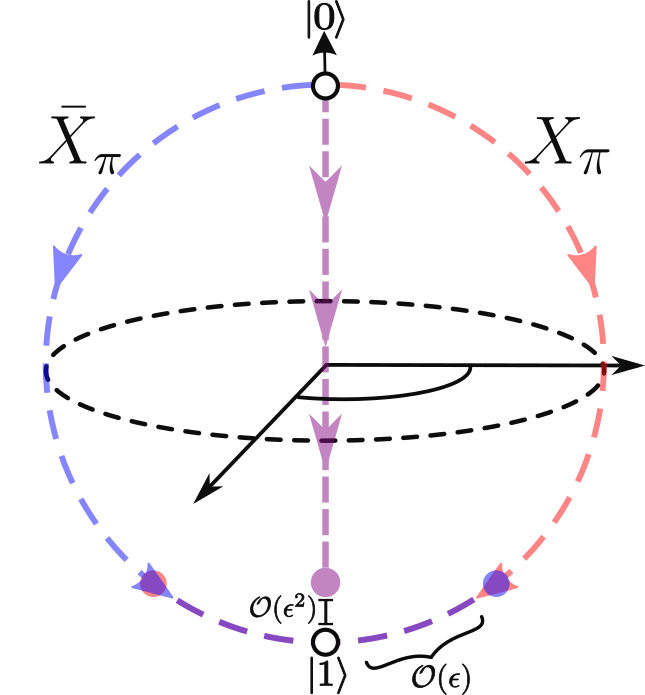
\includegraphics[width=.75\columnwidth]{simple_example.png}
  \caption{An example of a BCS. The red path is a $\pi$ pulse over-rotating clockwise, while the blue path is a $\pi$ pulse over-rotating counter-clockwise. The purple path is the average of the two.}
  \label{fig:simple_example}
\end{figure}

\section{A Simple Example}
As a somewhat trivial example, consider a single-qubit rotation-angle error, such as result from stochastic laser amplitude fluctuations. A BCS may consist of an $X_\pi$ pulse, as well as an $\bar X_\pi$ pulse (i.e., a clockwise and counter clockwise rotation of the qubit). In the case of excess amplitude, the $X_\pi$ pulse will result in an over-rotation error, while the $\bar X_\pi$ pulse results in an \emph{under}-rotation error. When it comes time to perform the target gate in a quantum circuit, one member of the BCS is chosen uniformly at random. This has the effect of decreasing the norm of the noise channel and decorrelating the over-rotation error (Figure \ref{fig:simple_example}). In this simple example, we can solve the minimization problem given by equation \ref{eq:minimization} analytically. In particular, if we choose the weights in \ref{eq:1} such that $\omega_i=1$, and we choose to represent ou gates in the vectorized superoperator representation, then:

\begin{equation}
  \begin{gathered}
    \frac{1}{2}(X_{\pi + \epsilon} + \bar X_{\pi + \epsilon}) \\  
    = (\sin^2{\frac{\pi + \epsilon}{2}}I + \cos^2{\frac{\pi + \epsilon}{2}}X)X \\
    \approx ((1 - \epsilon^2)I + \epsilon^2X)X
  \end{gathered}
\end{equation}
 
Therefore, for a rotational error of angle $\epsilon > 0$, we see that $X_\pi$ and  $\bar X_\pi$  form a BCS, with $\alpha\approx\epsilon^2$.


\section{1Q Gates}\label{1Q Gates}
 In this section, we present numerical results on generating one-qubit gates that together with $RZ(\theta$) rotations are universal for one-qubit computation. Our control Hamiltonian is given as: 
\begin{equation}\label{eq:1Qham}
  H = \epsilon\sigma_z + (1 + \delta)(c_x(t)\sigma_x + c_y(t)\sigma_y)
\end{equation}
$\epsilon$ is a normally distributed random variable, centered at $0$ with standard deviation $.001$, corresponding to a time varying Stark shift on the qubit. $\delta$ is also a normally distributed random variable with the same parameters, and is meant to represent random fluctuations in the control electronics, such as diurnal variations resulting from temperature instability. We assume that the errors on $\sigma_x$ and $\sigma_y$ are perfecly correlated, as mentioned in Section \ref{ocp}.
[ADD ANALYSIS OF PLOTS]
\begin{figure*}
\centering
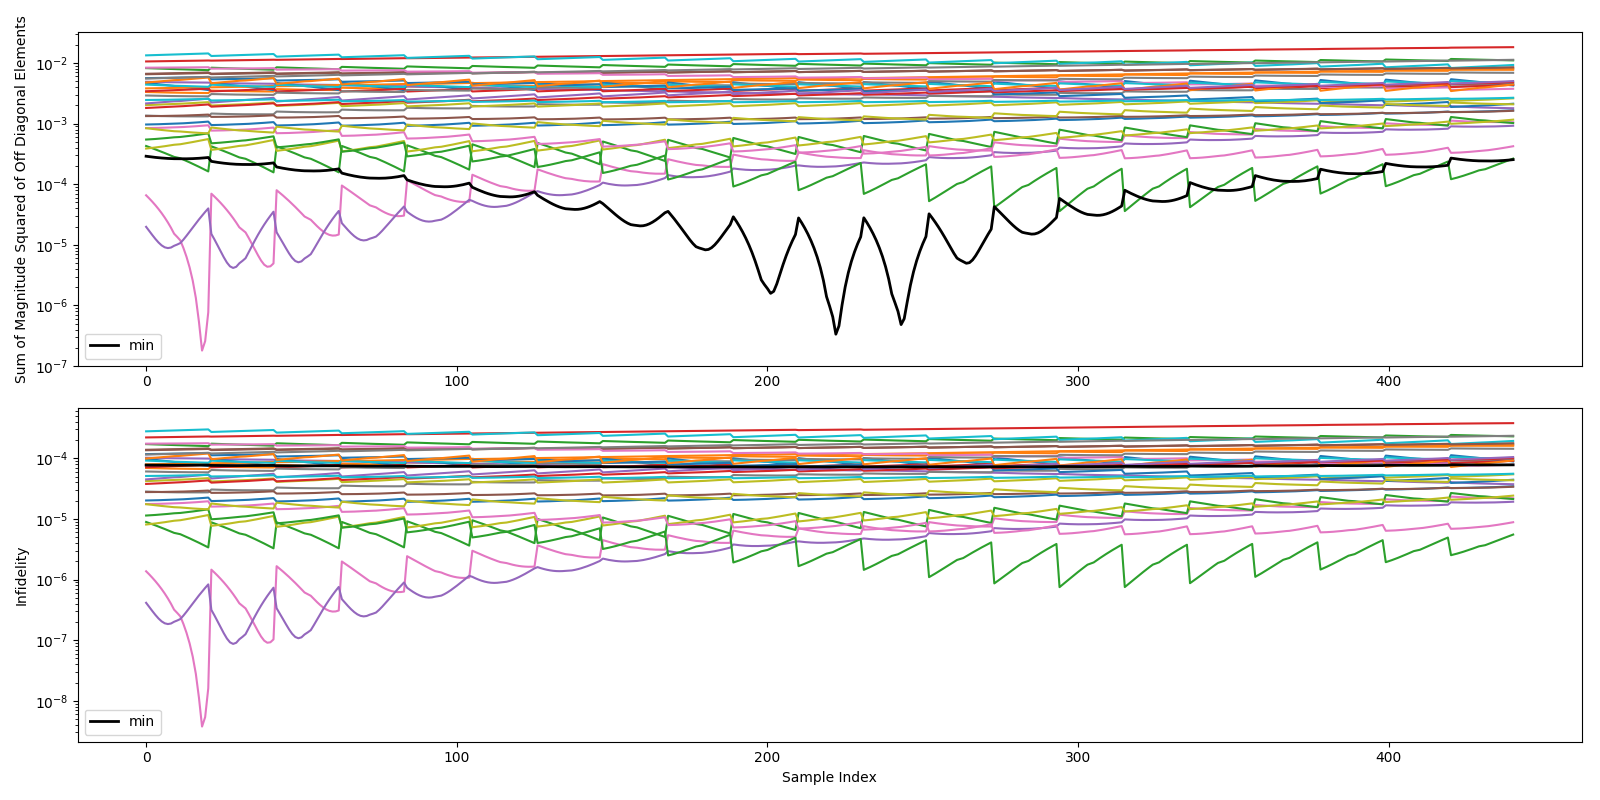
\includegraphics[width=\textwidth]{x2.png}
\caption{In the above we have used our method to produce a BCS for a $RX(\frac{\pi}{2})$ pulse, with the Hamiltonian given in \ref{eq:1Qham}. A) shows the sum of the squared norms of the off diagonal terms in the Pauli Transfer Matrix of $\mathcal{E}$. B) gives the corresponding infidelity for each member of the BCS, and the optimal choice of weights.}
\end{figure*}

\begin{figure*}
\centering
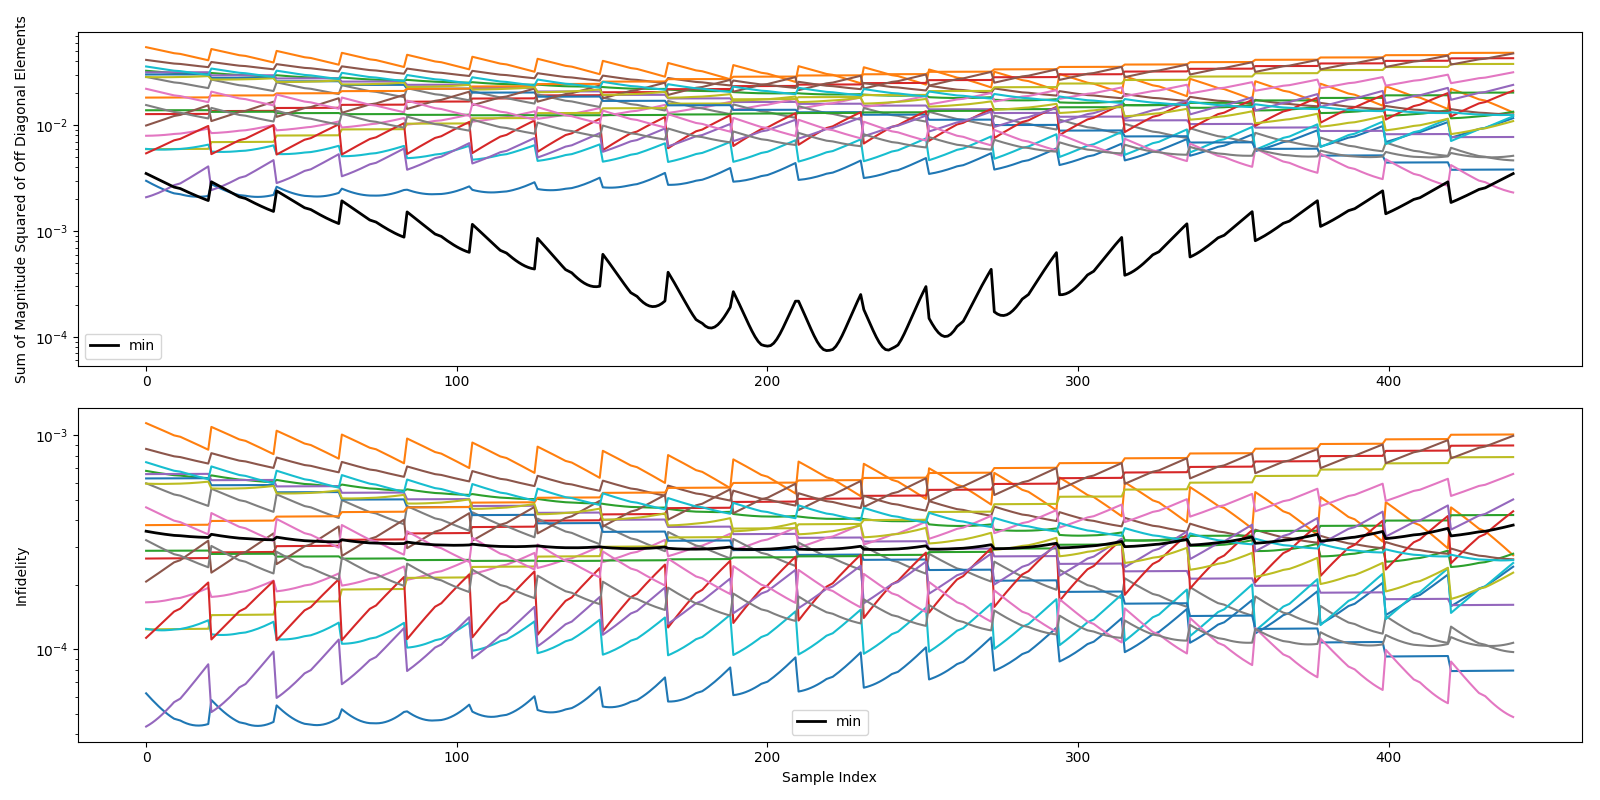
\includegraphics[width=\textwidth]{y2.png}
\caption{In the above we have used our method to produce a BCS for a $RY(\frac{\pi}{2})$ pulse, with the Hamiltonian given in \ref{eq:1Qham}. A) shows the sum of the squared norms of the off diagonal terms in the Pauli Transfer Matrix of $\mathcal{E}$. B) gives the corresponding infidelity for each member of the BCS, and the optimal choice of weights.}
\end{figure*}



\section{2Q Gates}\label{2Q Gates}
 In this section, we present numerical results on a generating one and two-qubit gates that together with $RZ(\theta)$ rotations are universal for two-qubit computation. Our control Hamiltonian is given as: 
\begin{equation} \label{eq:2Qham}
H = \exp{(-i\frac{\sigma_z^1\otimes\sigma_z^2}{4})} + \sum_{j=1}^2(\epsilon_j\sigma_z^j + (1 + \delta_j)(c_x^jx(t)\sigma_x^j + c_y^j(t)\sigma_y^j))
\end{equation}
We again assume that the standard deviations are $.001$ on all parameters $\delta_j$ and $c^j_i$ and that errors on the single qubit $\sigma_x$ and $\sigma_y$ rotations are perfectly correlated.
[ADD ANALYSIS OF PLOTS]
%These plots take a little while to make, so I can't iterate *that* fast - clearly the fonts need to be bigger, and there should be a title what else add a legend saying the black is the optimal?
\begin{figure*}[t]
\centering
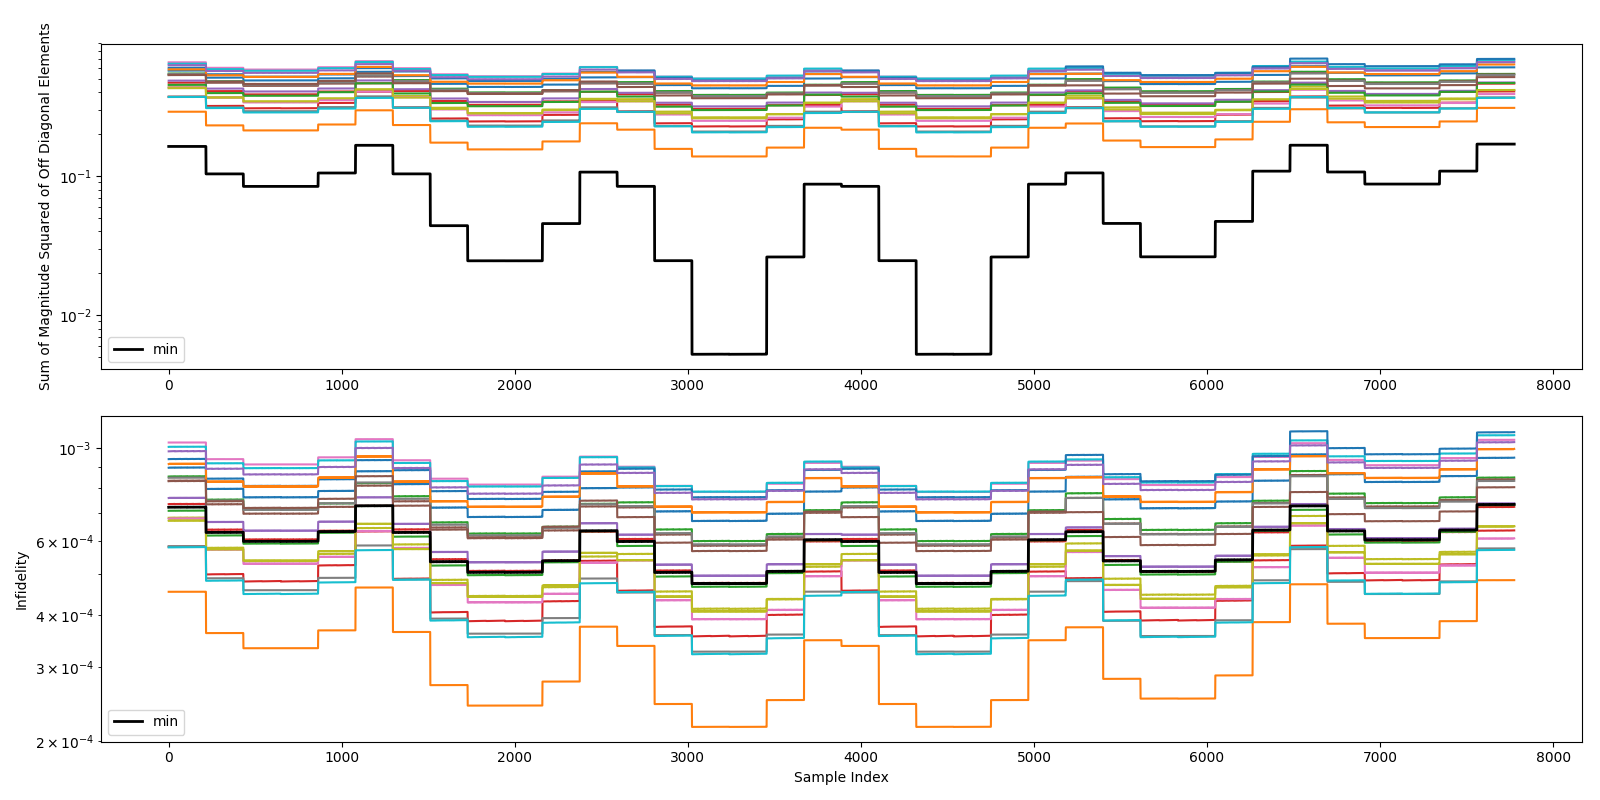
\includegraphics[width=\textwidth]{2Q.png}
\caption{In the above we have used our method to produce a BCS for a ZZ($\frac{\pi}{2}$) entangling gate with controls given by \ref{eq:2Qham}. A) shows the sum of the squared norms of the off diagonal terms in the Pauli Transfer Matrix of $\mathcal{E}$. B) gives the corresponding infidelity for each member of the BCS, and the optimal choice of weights.}
\end{figure*}








%It might be interesting to show a dhistogram of the pribabilities assigned to each control to show that they aren't all zero. and maybe 



%$$ \epsilon, \delta \midtilde \sim \mathcal{N}(0, .001) $$
%$$\epsilon_0, \epsilon_1, \delta_0, \delta_1 \midtilde \sim \mathcal{N}(0, .001)$$
\bibliography{decorrelation.bib}
\end{document}
